\begin{frame}[plain,c]
\begin{center}
	\huge Construction methods
\end{center}
\end{frame}

\begin{frame}
	\frametitle{How to create}
	\begin{itemize}
		\item Bose method
		\item Skolem
		\item $6n + 5$
		\item With quasigroups with holes
		\item Wilson
		\item $2n +1$
		\item $2n +7$
		\item Even-Odd
	\end{itemize}
\end{frame}

\begin{frame}
	\frametitle{Bose construction}
	We need first define:\\
	\textbf{idempotent commutative quasigroups of order $2n + 1$}
\end{frame}

%esprimiamo vari risultati che non sono inclusi in tutti i libri in quanto alcuni li danno per scontati 
\begin{frame}
	\frametitle{But first: recap}
	\begin{columns}
		\column{0.4\textwidth}
		\begin{block}{(Definition) latin square of order $n$}
			is an $n \times n$ array where each row and column contains all symbols $\{1,...,n\}$ exactly one time.
		\end{block}
	\begin{table}[]
		\begin{tabular}{cccll}
			\cline{1-3}
			\multicolumn{1}{|c|}{1} & \multicolumn{1}{c|}{3} & \multicolumn{1}{c|}{2} &  &  \\ \cline{1-3}
			\multicolumn{1}{|c|}{2} & \multicolumn{1}{c|}{1} & \multicolumn{1}{c|}{3} &  &  \\ \cline{1-3}
			\multicolumn{1}{|c|}{3} & \multicolumn{1}{c|}{2} & \multicolumn{1}{c|}{1} &  &  \\ \cline{1-3}
			\multicolumn{1}{l}{}    & \multicolumn{1}{l}{}   & \multicolumn{1}{l}{}   &  & 
		\end{tabular}
	\caption{Latin square of order $3$}
	\end{table}
	
		\column{0.4\textwidth}
		\begin{block}{(Definition) Quasigroup}
		A \textit{quasigroup} of \textit{order} $n$ is an algebric structure, a pair $(Q,\circ)$ where $|Q|=n$ and $\circ : Q \times Q \rightarrow Q$.\\ $\forall a,b \in Q$ then $\exists! x,y$ (unique!) to the equations $a \circ x = b$ and $x \circ a = b$. 
		\end{block}

		An examples of quasigroup are $(\mathrm{Z_n},-)$,$(\mathrm{Z_n},+)$.
	\end{columns}
\end{frame}

\begin{frame}
\frametitle{(Example) 1723 Latin square}
\pause[1]
\begin{figure}
	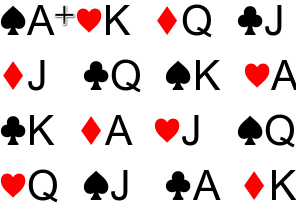
\includegraphics[width=0.3\textwidth]{figures_and_colours}
\end{figure}

\begin{columns}
	\column[]{0.5\textwidth}
	\pause[2]
	\begin{figure}
		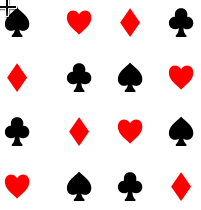
\includegraphics[width=0.5\textwidth]{colours}
	\end{figure}
	\column[]{0.5\textwidth}
	\pause[3]
	\begin{figure}
		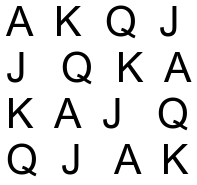
\includegraphics[width=0.5\textwidth]{figures}
	\end{figure}
	
\end{columns}
\end{frame}


\begin{frame}
\frametitle{Quasigroup and latin square}
%Theorem The multiplication table of a quasigroup is a  Latin square.

\begin{theorem}
	The multiplication table of a quasigroup is a  Latin square
\end{theorem}
A quasigroup $(G,\circ)$ is a latin square of order $v=|G|$:

	
	\begin{columns}
		\column{0.5\textwidth}
		\begin{table}[]
			\begin{tabular}{ccccc}
				\cline{1-3}
				\multicolumn{1}{|c|}{1} & \multicolumn{1}{c|}{3} & \multicolumn{1}{c|}{2} &  &  \\ \cline{1-3}
				\multicolumn{1}{|c|}{2} & \multicolumn{1}{c|}{1} & \multicolumn{1}{c|}{3} &  &  \\ \cline{1-3}
				\multicolumn{1}{|c|}{3} & \multicolumn{1}{c|}{2} & \multicolumn{1}{c|}{1} &  &  \\ \cline{1-3}
				\multicolumn{1}{l}{}    & \multicolumn{1}{l}{}   & \multicolumn{1}{l}{}   &  & 
			\end{tabular}
			\caption{Latin square of order $3$}
		\end{table}
		\column{0.5\textwidth}
		\begin{table}[]
			\begin{tabular}{ccccc}
				%\hline
				$\circ$				   & \multicolumn{1}{|c|}{1} & \multicolumn{1}{c|}{2} & \multicolumn{1}{c|}{3}  \\ \hline
				\multicolumn{1}{c|}{1} & \multicolumn{1}{c|}{1} & \multicolumn{1}{c|}{2} & \multicolumn{1}{c|}{3}  \\ \hline
				\multicolumn{1}{c|}{2} & \multicolumn{1}{c|}{3} & \multicolumn{1}{c|}{1} & \multicolumn{1}{c|}{2}  \\ \hline
				\multicolumn{1}{c|}{3} & \multicolumn{1}{c|}{2} & \multicolumn{1}{c|}{3} & \multicolumn{1}{c|}{1}  \\ \hline
			\end{tabular}
			\caption{Quasigroup of order $3$}
		\end{table}
	\end{columns}
	\pause
	A $(Q,\circ)$ is said:
	\begin{description}%una relazione d'ordine su G
		\item[idempotent] $\forall i : 1 \le i \le |G|$ the cell $(i,i)$ contains $\alpha$ such that $\alpha \le i$
		\item[commutative] $\forall i,j : 1 \le i<j \le |G|$ the cell $(i,j)$ contains the same of $(j,i)$
	\end{description}

\end{frame}


% esporre le proprietà commutativa e idempotente sull'esempio
\begin{frame}
\frametitle{Commutative idempotent latin square}
\begin{center}
	\begin{table}[]
		\begin{tabular}{|c|c|c|}
			\hline
			1 & 3 & 2 \\ \hline
			3 & 2 & 1 \\ \hline
			2 & 1 & 3 \\ \hline
		\end{tabular}
	\caption{C. I. latin square of order $3$}
	\end{table}
\end{center}
\pause
%proviamo a pensare in modo naive ? 
\textcolor{red}{How can we create a \textit{C.I. latinsquare/quasigroup of order v} ?}
\end{frame}

\begin{frame}
\frametitle{contenuto...}
\begin{theorem}%l'idea è quella di non poter scaricare il carico in modo simmetrico o di rispettare la prop principale del latin square
	idempotent commutative quasigroups exist \textbf{if and only if} they have \textit{odd} order.
\end{theorem}

Great! We look at the half of all possible
\end{frame}

\begin{frame}
\frametitle{Construction method of CI quasigroup}
\begin{enumerate}
	\item Let $v$ be the order of quasigroup, take $(Z_v,+)$ where $+$ is the addition in $Z_v$.
	\item For all element $i := i +1$
	\item Take the elements of main diagonal $<d_1,...,d_v>$. Build a permutation $\sigma_v = \{(d_1,1), (d_2,2),..., (d_v,v)\}$.
	\item Apply $\sigma_v$ for all element of the \textit{multiplication table}
\end{enumerate}
As result you have a CI quasigroup.
\end{frame}

%a formal method, because a permutation of a correct row perform a correct row too. A left rotation $v$ times give you $v$ different element. So a bijective trasformation doesn't change this property.
\begin{frame}
\frametitle{Construction method of CI quasigroup of order 7}
\begin{columns}
	
	\column{0.5\textwidth}
	\begin{table}[]
		\begin{tabular}{llllllll}
			$Z_7$,+                 & 0                      & 1                      & 2                      & 3                      & 4                      & 5                      & 6                      \\ \cline{2-8} 
			\multicolumn{1}{l|}{0} & \multicolumn{1}{l|}{0} & \multicolumn{1}{l|}{1} & \multicolumn{1}{l|}{2} & \multicolumn{1}{l|}{3} & \multicolumn{1}{l|}{4} & \multicolumn{1}{l|}{5} & \multicolumn{1}{l|}{6} \\ \cline{2-8} 
			\multicolumn{1}{l|}{1} & \multicolumn{1}{l|}{1} & \multicolumn{1}{l|}{2} & \multicolumn{1}{l|}{3} & \multicolumn{1}{l|}{4} & \multicolumn{1}{l|}{5} & \multicolumn{1}{l|}{6} & \multicolumn{1}{l|}{0} \\ \cline{2-8} 
			\multicolumn{1}{l|}{2} & \multicolumn{1}{l|}{2} & \multicolumn{1}{l|}{3} & \multicolumn{1}{l|}{4} & \multicolumn{1}{l|}{5} & \multicolumn{1}{l|}{6} & \multicolumn{1}{l|}{0} & \multicolumn{1}{l|}{1} \\ \cline{2-8} 
			\multicolumn{1}{l|}{3} & \multicolumn{1}{l|}{3} & \multicolumn{1}{l|}{4} & \multicolumn{1}{l|}{5} & \multicolumn{1}{l|}{6} & \multicolumn{1}{l|}{0} & \multicolumn{1}{l|}{1} & \multicolumn{1}{l|}{2} \\ \cline{2-8} 
			\multicolumn{1}{l|}{4} & \multicolumn{1}{l|}{4} & \multicolumn{1}{l|}{5} & \multicolumn{1}{l|}{6} & \multicolumn{1}{l|}{0} & \multicolumn{1}{l|}{1} & \multicolumn{1}{l|}{2} & \multicolumn{1}{l|}{3} \\ \cline{2-8} 
			\multicolumn{1}{l|}{5} & \multicolumn{1}{l|}{5} & \multicolumn{1}{l|}{6} & \multicolumn{1}{l|}{0} & \multicolumn{1}{l|}{1} & \multicolumn{1}{l|}{2} & \multicolumn{1}{l|}{3} & \multicolumn{1}{l|}{4} \\ \cline{2-8} 
			\multicolumn{1}{l|}{6} & \multicolumn{1}{l|}{6} & \multicolumn{1}{l|}{0} & \multicolumn{1}{l|}{1} & \multicolumn{1}{l|}{2} & \multicolumn{1}{l|}{3} & \multicolumn{1}{l|}{4} & \multicolumn{1}{l|}{5} \\ \cline{2-8} 
		\end{tabular}
	\end{table}

	\column{0.5\textwidth}
		\begin{table}[]
		\begin{tabular}{llllllll}
			& 1                      & 2                      & 3                      & 4                      & 5                      & 6                      & 7                      \\ \cline{2-8} 
			\multicolumn{1}{l|}{1} & \multicolumn{1}{l|}{1} & \multicolumn{1}{l|}{2} & \multicolumn{1}{l|}{3} & \multicolumn{1}{l|}{4} & \multicolumn{1}{l|}{5} & \multicolumn{1}{l|}{6} & \multicolumn{1}{l|}{7} \\ \cline{2-8} 
			\multicolumn{1}{l|}{2} & \multicolumn{1}{l|}{2} & \multicolumn{1}{l|}{3} & \multicolumn{1}{l|}{4} & \multicolumn{1}{l|}{5} & \multicolumn{1}{l|}{6} & \multicolumn{1}{l|}{7} & \multicolumn{1}{l|}{1} \\ \cline{2-8} 
			\multicolumn{1}{l|}{3} & \multicolumn{1}{l|}{3} & \multicolumn{1}{l|}{4} & \multicolumn{1}{l|}{5} & \multicolumn{1}{l|}{6} & \multicolumn{1}{l|}{7} & \multicolumn{1}{l|}{1} & \multicolumn{1}{l|}{2} \\ \cline{2-8} 
			\multicolumn{1}{l|}{4} & \multicolumn{1}{l|}{4} & \multicolumn{1}{l|}{5} & \multicolumn{1}{l|}{6} & \multicolumn{1}{l|}{7} & \multicolumn{1}{l|}{1} & \multicolumn{1}{l|}{2} & \multicolumn{1}{l|}{3} \\ \cline{2-8} 
			\multicolumn{1}{l|}{5} & \multicolumn{1}{l|}{5} & \multicolumn{1}{l|}{6} & \multicolumn{1}{l|}{7} & \multicolumn{1}{l|}{1} & \multicolumn{1}{l|}{2} & \multicolumn{1}{l|}{3} & \multicolumn{1}{l|}{4} \\ \cline{2-8} 
			\multicolumn{1}{l|}{6} & \multicolumn{1}{l|}{6} & \multicolumn{1}{l|}{7} & \multicolumn{1}{l|}{1} & \multicolumn{1}{l|}{2} & \multicolumn{1}{l|}{3} & \multicolumn{1}{l|}{4} & \multicolumn{1}{l|}{5} \\ \cline{2-8} 
			\multicolumn{1}{l|}{7} & \multicolumn{1}{l|}{7} & \multicolumn{1}{l|}{1} & \multicolumn{1}{l|}{2} & \multicolumn{1}{l|}{3} & \multicolumn{1}{l|}{4} & \multicolumn{1}{l|}{5} & \multicolumn{1}{l|}{6} \\ \cline{2-8} 
		\end{tabular}
	\end{table}
\end{columns}

\begin{enumerate}
	\item Let $v$ be the order of quasigroup, take $(Z_v,+)$ where $+$ is the addition in $Z_v$.
	\item For all element $i := i +1$
\end{enumerate}
\end{frame}


\begin{frame}
\frametitle{Construction method of CI quasigroup of order 7}
\begin{columns}
	\column{0.5\textwidth}
	\begin{table}[]
		\begin{tabular}{ccccccccc}
			& 1                      & 2                      & 3                      & 4                      & 5                      & 6                      & 7                      \\ \cline{2-8} 
			\multicolumn{1}{l|}{1} & \multicolumn{1}{l|}{1} & \multicolumn{1}{l|}{2} & \multicolumn{1}{l|}{3} & \multicolumn{1}{l|}{4} & \multicolumn{1}{l|}{5} & \multicolumn{1}{l|}{6} & \multicolumn{1}{l|}{7} \\ \cline{2-8} 
			\multicolumn{1}{l|}{2} & \multicolumn{1}{l|}{2} & \multicolumn{1}{l|}{3} & \multicolumn{1}{l|}{4} & \multicolumn{1}{l|}{5} & \multicolumn{1}{l|}{6} & \multicolumn{1}{l|}{7} & \multicolumn{1}{l|}{1} \\ \cline{2-8} 
			\multicolumn{1}{l|}{3} & \multicolumn{1}{l|}{3} & \multicolumn{1}{l|}{4} & \multicolumn{1}{l|}{5} & \multicolumn{1}{l|}{6} & \multicolumn{1}{l|}{7} & \multicolumn{1}{l|}{1} & \multicolumn{1}{l|}{2} \\ \cline{2-8} 
			\multicolumn{1}{l|}{4} & \multicolumn{1}{l|}{4} & \multicolumn{1}{l|}{5} & \multicolumn{1}{l|}{6} & \multicolumn{1}{l|}{7} & \multicolumn{1}{l|}{1} & \multicolumn{1}{l|}{2} & \multicolumn{1}{l|}{3} \\ \cline{2-8} 
			\multicolumn{1}{l|}{5} & \multicolumn{1}{l|}{5} & \multicolumn{1}{l|}{6} & \multicolumn{1}{l|}{7} & \multicolumn{1}{l|}{1} & \multicolumn{1}{l|}{2} & \multicolumn{1}{l|}{3} & \multicolumn{1}{l|}{4} \\ \cline{2-8} 
			\multicolumn{1}{l|}{6} & \multicolumn{1}{l|}{6} & \multicolumn{1}{l|}{7} & \multicolumn{1}{l|}{1} & \multicolumn{1}{l|}{2} & \multicolumn{1}{l|}{3} & \multicolumn{1}{l|}{4} & \multicolumn{1}{l|}{5} \\ \cline{2-8} 
			\multicolumn{1}{l|}{7} & \multicolumn{1}{l|}{7} & \multicolumn{1}{l|}{1} & \multicolumn{1}{l|}{2} & \multicolumn{1}{l|}{3} & \multicolumn{1}{l|}{4} & \multicolumn{1}{l|}{5} & \multicolumn{1}{l|}{6} \\ \cline{2-8} 
		\end{tabular}
	\end{table}
	\column{0.5\textwidth}
	$\sigma_v = \{ (1,1), (3,2), (5,3),$ \\
	$ \quad (7,4), (2,5), (4,6), (6,7) \}$
\end{columns}

\begin{enumerate}
	\item Let $v$ be the order of quasigroup, take $(Z_v,+)$ where $+$ is the addition in $Z_v$.
	\item For all element $i := i +1$
	\item Take the elements of main diagonal $<d_1,...,d_v>$. Build a permutation $\sigma_v = \{(d_1,1), (d_2,2),..., (d_v,v)\}$.
	\item Apply $\sigma_v$ for all element of the \textit{multiplication table}
\end{enumerate}
\end{frame}


\begin{frame}
\frametitle{Construction method of CI quasigroup of order 7}
\begin{columns}
	\column{0.5\textwidth}
	\begin{table}[]
		\begin{tabular}{cccccccc}
			& 1                      & 2                      & 3                      & 4                      & 5                      & 6                      & 7                      \\ \cline{2-8} 
			\multicolumn{1}{l|}{1} & \multicolumn{1}{l|}{1} & \multicolumn{1}{l|}{2} & \multicolumn{1}{l|}{3} & \multicolumn{1}{l|}{4} & \multicolumn{1}{l|}{5} & \multicolumn{1}{l|}{6} & \multicolumn{1}{l|}{7} \\ \cline{2-8} 
			\multicolumn{1}{l|}{2} & \multicolumn{1}{l|}{2} & \multicolumn{1}{l|}{3} & \multicolumn{1}{l|}{4} & \multicolumn{1}{l|}{5} & \multicolumn{1}{l|}{6} & \multicolumn{1}{l|}{7} & \multicolumn{1}{l|}{1} \\ \cline{2-8} 
			\multicolumn{1}{l|}{3} & \multicolumn{1}{l|}{3} & \multicolumn{1}{l|}{4} & \multicolumn{1}{l|}{5} & \multicolumn{1}{l|}{6} & \multicolumn{1}{l|}{7} & \multicolumn{1}{l|}{1} & \multicolumn{1}{l|}{2} \\ \cline{2-8} 
			\multicolumn{1}{l|}{4} & \multicolumn{1}{l|}{4} & \multicolumn{1}{l|}{5} & \multicolumn{1}{l|}{6} & \multicolumn{1}{l|}{7} & \multicolumn{1}{l|}{1} & \multicolumn{1}{l|}{2} & \multicolumn{1}{l|}{3} \\ \cline{2-8} 
			\multicolumn{1}{l|}{5} & \multicolumn{1}{l|}{5} & \multicolumn{1}{l|}{6} & \multicolumn{1}{l|}{7} & \multicolumn{1}{l|}{1} & \multicolumn{1}{l|}{2} & \multicolumn{1}{l|}{3} & \multicolumn{1}{l|}{4} \\ \cline{2-8} 
			\multicolumn{1}{l|}{6} & \multicolumn{1}{l|}{6} & \multicolumn{1}{l|}{7} & \multicolumn{1}{l|}{1} & \multicolumn{1}{l|}{2} & \multicolumn{1}{l|}{3} & \multicolumn{1}{l|}{4} & \multicolumn{1}{l|}{5} \\ \cline{2-8} 
			\multicolumn{1}{l|}{7} & \multicolumn{1}{l|}{7} & \multicolumn{1}{l|}{1} & \multicolumn{1}{l|}{2} & \multicolumn{1}{l|}{3} & \multicolumn{1}{l|}{4} & \multicolumn{1}{l|}{5} & \multicolumn{1}{l|}{6} \\ \cline{2-8} 
		\end{tabular}
	\end{table}
	\column{0.5\textwidth}
		\begin{table}[]
		\begin{tabular}{cccccccc}
			& 1                      & 2                      & 3                      & 4                      & 5                      & 6                      & 7                      \\ \cline{2-8} 
			\multicolumn{1}{l|}{1} & \multicolumn{1}{l|}{1} & \multicolumn{1}{l|}{5} & \multicolumn{1}{l|}{2} & \multicolumn{1}{l|}{6} & \multicolumn{1}{l|}{3} & \multicolumn{1}{l|}{7} & \multicolumn{1}{l|}{4} \\ \cline{2-8} 
			\multicolumn{1}{l|}{5} & \multicolumn{1}{l|}{5} & \multicolumn{1}{l|}{2} & \multicolumn{1}{l|}{6} & \multicolumn{1}{l|}{3} & \multicolumn{1}{l|}{7} & \multicolumn{1}{l|}{4} & \multicolumn{1}{l|}{1} \\ \cline{2-8} 
			\multicolumn{1}{l|}{2} & \multicolumn{1}{l|}{2} & \multicolumn{1}{l|}{6} & \multicolumn{1}{l|}{3} & \multicolumn{1}{l|}{7} & \multicolumn{1}{l|}{4} & \multicolumn{1}{l|}{1} & \multicolumn{1}{l|}{5} \\ \cline{2-8} 
			\multicolumn{1}{l|}{6} & \multicolumn{1}{l|}{6} & \multicolumn{1}{l|}{3} & \multicolumn{1}{l|}{7} & \multicolumn{1}{l|}{4} & \multicolumn{1}{l|}{1} & \multicolumn{1}{l|}{5} & \multicolumn{1}{l|}{2} \\ \cline{2-8} 
			\multicolumn{1}{l|}{3} & \multicolumn{1}{l|}{3} & \multicolumn{1}{l|}{7} & \multicolumn{1}{l|}{4} & \multicolumn{1}{l|}{1} & \multicolumn{1}{l|}{5} & \multicolumn{1}{l|}{2} & \multicolumn{1}{l|}{6} \\ \cline{2-8} 
			\multicolumn{1}{l|}{7} & \multicolumn{1}{l|}{7} & \multicolumn{1}{l|}{4} & \multicolumn{1}{l|}{1} & \multicolumn{1}{l|}{5} & \multicolumn{1}{l|}{2} & \multicolumn{1}{l|}{6} & \multicolumn{1}{l|}{3} \\ \cline{2-8} 
			\multicolumn{1}{l|}{4} & \multicolumn{1}{l|}{4} & \multicolumn{1}{l|}{1} & \multicolumn{1}{l|}{5} & \multicolumn{1}{l|}{2} & \multicolumn{1}{l|}{6} & \multicolumn{1}{l|}{3} & \multicolumn{1}{l|}{7} \\ \cline{2-8} 
		\end{tabular}
	\end{table}
\end{columns}
	We apply $\sigma_v = \{ (1,1), (3,2), (5,3),(7,4), (2,5), (4,6), (6,7) \}$ as result we have a idempotent commutative quasigroup of order $v$.
\end{frame}

\begin{frame}
\frametitle{Bose construction($v \equiv 3 mod(6)$)} 
Let $v = 6n +3$ and let $(Q,\circ)$ be an idempotent commutative quasigroup of order $2n+1$, where $Q = \{1,2,3,...,2n+1\}$. Let $S= Q \times \{1,2,3\}$ and define $T$ to contain the following types of triples.
\begin{description}
	\item[Type 1:] For $1 \le i \le 2n +1, \ \{(i,1),(i,2),(i,3)\} \in T$ 
	\item[Type 2:] For $1 \le i < j \le 2n +1, \ \{ \{ (i,1),(j,1),(i \circ j,2)\},\{ (i,2),(j,2),(i \circ j,3)\}\{ (i,3),(j,3),(i \circ j,1)\}\} \in T$
\end{description}

Then $(S,T)$ is a Steiner triple system of order $6n + 3$.

\end{frame}

\begin{frame}
\frametitle{Type of partitions}
\begin{figure}
	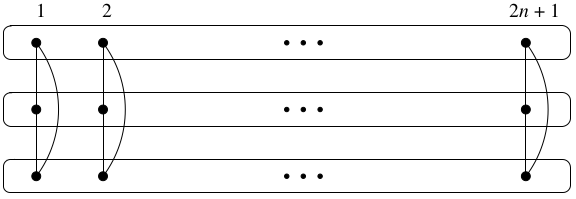
\includegraphics[width=0.7\textwidth]{bose_1}
	\caption{Type 1}
\end{figure}
\begin{figure}
	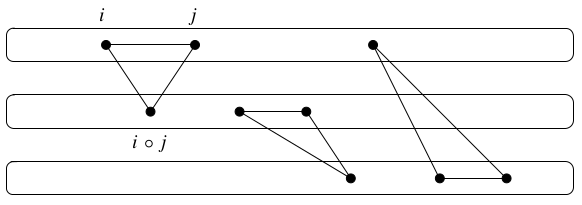
\includegraphics[width=0.7\textwidth]{bose_2}
	\caption{Type 2}
\end{figure}
\end{frame}


\begin{comment}
If we are considering a set of v(v-1)/6 triples of 
elements of a v-set and know that each pair elements is 
contained in at least one triple, then each pair must be 
contained in exactly one triple and we have an STS(v). 
Therefore we need only count the number of triples and verify 
that each pair of elements is contained in a triple in order to 
show that a system is an STS.
\end{comment}
\begin{frame}
\frametitle{Proof}
%we need to prove that all pairs are v(v-1)/6 then, as result of all pair is contained only one, we have proved the corecteness.
$|T|$ is made up with 2 type:
\begin{itemize}
	\item \textit{Type 1}: $2n+1$ triples
	\item \textit{Type 2}: $\binom{2n + 1}{2}$ choices for $i$ and $j$, for all of them there are 3 another type.
\end{itemize} 
Then $|T| = (2n+1) + 3\frac{(2n+1)2n}{2} = \frac{(2n+1)(6n+2)}{2} = v(v-1)/6$ have the right number of triple.\\%I've used 

To show that every pairs is contained in at least 1 triple, think about 2 possible pair of point $(a,b),(c,d) \in Q \times \{1,2,3\}$:
\end{frame}

\begin{frame}
\frametitle{Cont..}
%e' distorta la notazione di punto in quanto dobbiamo pensare alla coppia di punti come una coppia di coppia di punti (siamo nella costruzione di Bose)
$\forall (a,b),(c,d) \in Q \times \{1,2,3\}$
\begin{itemize}
	\item $a=c \wedge b=d$ impossible
	\item if $a=c$ (so $b\not = d$) is contained in at least 1 triple of \textit{type 1} $\{\{(a,1),(a,2),(a,3)\}, \{(x,1),(a,1),(b,2)\}, ... \}$
	\item if $b=d \wedge a \not = c$ impossible) is contained in at least 1 triple of \textit{type 2} $\{\{(a,b),(c,b),(a \circ c, b+1 mod(3)\ )\}, \{(x,1),(a,1),(b,2)\}, ... \}$
	\item $a \not = c \wedge b \not = d$.%assume for example. The other can be produced by iteration on the 6 pair from the 3 possible partition 
	Assume $b=1$ and $d=2$. Since $(Q,\circ)$ is a quasigroup $a \circ i = c$ and $j \circ a = c$ for some $i,j$. Because the \textit{commutative} $i=j$ and because \textit{idempotent} only $a \circ a=a$, all the others we are sure that $i\not = a$. So $\{(a,1),(i,1),(a \circ i = c, 2)\}$.
\end{itemize}

All possible point have been shown that are in $T$.
\end{frame}

\begin{frame}
\frametitle{Example Bose construction}
\begin{figure}
	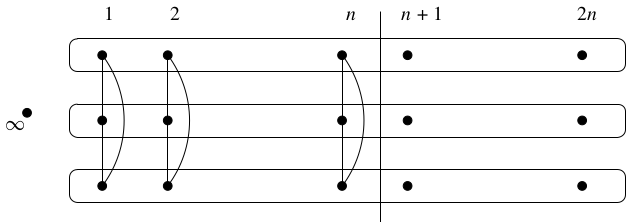
\includegraphics[height=0.2\textheight]{skolem_1}
	\begin{columns}
		\column[]{0.2\textwidth}
		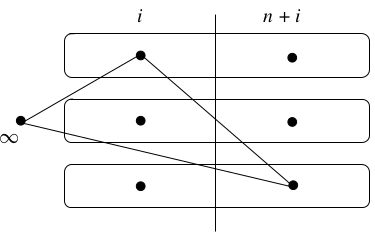
\includegraphics[height=0.2\textheight]{skolem_2_a}
		\column[]{0.1\textwidth}
		\column[]{0.2\textwidth}
		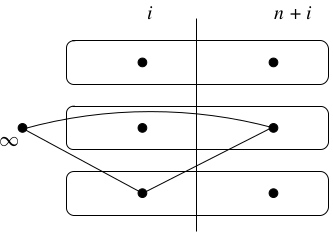
\includegraphics[height=0.2\textheight]{skolem_2_b}
		\column[]{0.1\textwidth}
		\column[]{0.2\textwidth}
		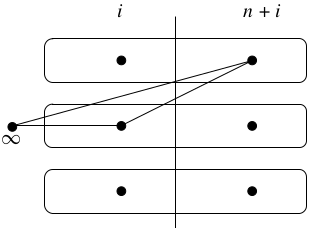
\includegraphics[height=0.2\textheight]{skolem_2_c}
	\end{columns}
	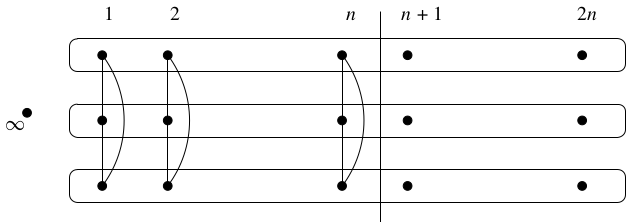
\includegraphics[height=0.2\textheight]{skolem_3}
\end{figure}
\end{frame}

\begin{frame}
\frametitle{Skolem construction ($v \equiv 3 mod(6)$)}
Let $v = 6n +1$ and let $(Q, \circ)$ be a half-idempotent commutative quasigroup of order $2n$, where ....
\end{frame}



\begin{frame}
\frametitle{Half-idempotent commutative latin square}

\begin{block}{(Definition)Half-idempotent commutative latin square}
A latin square (multiplication table of quasigroup of the same order) $L$ of order $2n$ is \textit{half-idempotent} if the cells $(i,i)$ contain the same symbol $i$ of the cell $(n+i,n+i)\quad \forall 1 \le i \le n$
\end{block}
\begin{columns}
	\column[]{0.5\textwidth}
	
	\begin{table}
		\centering
		\begin{tabular}{|l|l|l|l|} 
			\hline
			1 & 3 & 2 & 4  \\ 
			\hline
			3 & 2 & 4 & 1  \\ 
			\hline
			2 & 4 & 1 & 3  \\ 
			\hline
			4 & 1 & 3 & 2  \\
			\hline
		\end{tabular}
	\end{table}
	\column[]{0.4\textwidth}
	Half-idempotent latin square of order $4$ ($n=2$)
	
	\column[]{0.1\textwidth}
\end{columns}

\pause
\setbeamercolor{block title}{bg=green!30,fg=black!20}
\begin{block}{}
	\textit{Commutative half-idempotent latin squares} exist for all \textit{even} order.
\end{block}

\end{frame}

\begin{frame}
\frametitle{Example half-idempotent quasigroup}

\begin{columns}
	\column[]{0.5\textwidth}
	\begin{table}
		\centering
		\begin{tabular}{|l|l|l|l|} 
			\hline
			1 & 3 & 2 & 4  \\ 
			\hline
			3 & 2 & 4 & 1  \\ 
			\hline
			2 & 4 & 1 & 3  \\ 
			\hline
			4 & 1 & 3 & 2  \\
			\hline
		\end{tabular}
	\end{table}
	\column[]{0.5\textwidth}
	\begin{table}
		\centering
		\begin{tabular}{|l|l|l|l|l|l|} 
			\hline
			1 & 4 & 2 & 5 & 3 & 6                       \\ 
			\hline
			4 & 2 & 5 & 3 & 6 & 1                       \\ 
			\hline
			2 & 5 & 3 & 6 & 1 & 4                       \\ 
			\hline
			5 & 3 & 6 & 1 & 4 & 2                       \\ 
			\hline
			3 & 6 & 1 & 4 & 2 & 5                       \\ 
			\hline
			6 & 1 & 4 & 2 & 5 & \multicolumn{1}{c|}{3}  \\
			\hline
		\end{tabular}
	\end{table}
	
\end{columns}
\pause
\textcolor{red}{How can we algorithmically build a H-I Latin Square?}
\end{frame}



\begin{frame}
\frametitle{How costruct H-I latin square/quasigroup}

\begin{columns}
	\pause[1]
	\column[]{0.5\textwidth}
	\begin{table}
		\centering
		\begin{tabular}{|l|l|l|l|l|l|} 
			\hline
			0 & 1 & 2 & 3 & 4 & 5                       \\ 
			\hline
			1 & 2 & 3 & 4 & 5 & 0                       \\ 
			\hline
			2 & 3 & 4 & 5 & 0 & 1                       \\ 
			\hline
			3 & 4 & 5 & 0 & 1 & 2                       \\ 
			\hline
			4 & 5 & 0 & 1 & 2 & 3                       \\ 
			\hline
			5 & 0 & 1 & 2 & 3 & \multicolumn{1}{c|}{4}  \\
			\hline
		\end{tabular}
	\caption{Quasigroup $(\mathrm{Z}_6, + mod(6))$}
	\end{table}

	\pause[3]
	\column[]{0.5\textwidth}
	\begin{table}
		\centering
		\begin{tabular}{|l|l|l|l|l|l|} 
			\hline
			1 & 4 & 2 & 5 & 3 & 6                       \\ 
			\hline
			4 & 2 & 5 & 3 & 6 & 1                       \\ 
			\hline
			2 & 5 & 3 & 6 & 1 & 4                       \\ 
			\hline
			5 & 3 & 6 & 1 & 4 & 2                       \\ 
			\hline
			3 & 6 & 1 & 4 & 2 & 5                       \\ 
			\hline
			6 & 1 & 4 & 2 & 5 & \multicolumn{1}{c|}{3}  \\
			\hline
		\end{tabular}
	
	\caption{Applied func $\sigma$ on the quasigroup}
	\end{table}
	
\end{columns}

\pause[2]
The bijection $\sigma$ is built increasing all value by $1$(or by taking the next element). Then by taking the main diagonal from the left grid ($<1,3,5,...>$) and assign the right number ($<1,2,3,...>$) 
\end{frame}



\begin{frame}
\frametitle{Example Skolem construction}
Let $v = 6n +1$ and let $(Q, \circ)$ be a half-idempotent commutative quasigroup of order $2n$, where $Q = \{ 1,2,3,...., 2n\}$. Let $S = \{\infty\} \cup(Q \times \{1,2,3\})$. We define $T$ as follow:

\begin{description}
	\item[Type 1]: for $1 \le i \le n$, $\{ (i,1), (i,2), (i,3) \} \in T$ 
	\item[Type 2]: for $1 \le i \le n$ , $\{ \infty, (n+i,3),(i,2) \},\{ \infty, (n+i,2),(n+i,3) \},\{\infty,(n+i,3),(i,1) \} \in T$
	\item[Type 3]: for $1 \le i < j \le 2n$,$\{(i,1),(j,1),(i \circ j,2) \}, \{(i,2),(j,2),(i \circ j,3)\},\{\} \in T$
\end{description}
\end{frame}


\begin{frame}
We have to prove (in a similar way of Bose) there are the right number of $t \in T$ and every pair (from $\binom{6n + 1}{2}$) is contained almost 1.
\begin{proof}[1: Right number of $|T|$]
We sum up 3 different element:
\begin{itemize}
	\item \textit{type 1}: \textcolor{black!55}{for $1 \le i \le n$, $\{ (i,1), (i,2), (i,3)\} \in T$} are $n$
	\item \textit{type 2}: \textcolor{black!55}{ for $1 \le i \le n$ , $\{\infty, (n+i,3),(i,2)\},\{\infty,(n+i,2),(n+i,3)\},\{\infty,(n+i,3),(i,1) \} \in T$} are $3n$
	\item \textit{type 3}: \textcolor{black!55}{for $1 \le i < j \le 2n$,$\{(i,1),(j,1),(i \circ j,2) \}, \{(i,2),(j,2),(i \circ j,3)\},\{\} \in T$} are $3\binom{2n}{2}$
\end{itemize}
We have to prove $|T|= \frac{v(v-1)}{6} = \frac{(6n+1)(6n)}{6}= n + n + 3\binom{2n}{2}$.\\
Easily $n + 3n + 3\binom{2n}{2}=\frac{2n*4+ 2n*(6n-3)}{2}= \frac{2n(6n +1 )}{2}= \frac{3}{3}\frac{2n(6n +1 )}{2}=\frac{6n(6n +1 )}{2}=|T|$
\end{proof}
\end{frame}

\begin{frame}
\begin{proof}[2: every pair of point $\in T$]
	We have to prove all possible pair of point $(a,b)$ and $(c,d)$:
	\begin{itemize}
		\item $a=c=\infty \wedge b \not = d$
		\item $a=c\not = \infty \wedge b \not = d$
		\item $a= \infty \not = b \wedge b = d$
		\item $a\not =c \wedge b \not = d $
	\end{itemize}
\end{proof}
\pause
\setbeamercolor{block title}{bg=green!30,fg=black!20}
\begin{block}{}
All covered by Skolem construction $\wedge$ $|T|$ is the right number $\Rightarrow$ is a STS($2n$)
\end{block}

\end{frame}

